
\section{Constituencies and Counties}

\begin{enumerate}
\def\labelenumi{\arabic{enumi}.}
\itemsep1pt\parskip0pt\parsep0pt
\item
  About Wahlkreise and Landkreise
\item
  Configuration and Visualization in QGIS Desktop
\item
  Setup for Postgres (+Postgis)
\item
  Derivation of \emph{County} \textless{}-\textgreater{}
  \emph{Constituency}
\end{enumerate}

\subsection{About Wahlkreise and
Landkreise}\label{about-wahlkreise-and-landkreise}

Landkreise (counties) and Wahlkreise (constituencies) have different borders.
One does not contain the other. In order to understand the problem it is
recommended to configure and visualize the map in QGIS.

\subsection{Configuration and Visualization in QGIS
Desktop}\label{configuration-and-visualization-in-qgis-desktop}

\subsubsection{Requirements}\label{requirements}

Available Layers

\begin{itemize}
\itemsep1pt\parskip0pt\parsep0pt
\item
	\href{http://www.bundeswahlleiter.de/en/bundestagswahlen/BTW_BUND_13/wahlkreiseinteilung/kartographische_darstellung.html}{Wahlkreise}

	\begin{itemize}
	\itemsep1pt\parskip0pt\parsep0pt
	\item 
	Download:
	\href{http://www.bundeswahlleiter.de/de/bundestagswahlen/BTW_BUND_13/wahlkreiseinteilung/wahlkreisgeometrie/Geometrie_Wahlkreise_18DBT_VG1000_ETRS89.zip}{SHP}
	\item
	Projection: \textbf{EPSG:3044 - ETRS89 / ETRS-TM32}

\end{itemize}

\item
	\href{http://www.gadm.org/country}{Landkreise}
	
	\begin{itemize}
	\itemsep1pt\parskip0pt\parsep0pt
	\item 
	Download: \href{http://biogeo.ucdavis.edu/data/gadm2/shp/DEU_adm.zip}{SHP}
	\item
	Projection: \textbf{EPSG:4326 - WGS84}
	\end{itemize}

\end{itemize}
\subsubsection{Visualization}\label{visualization}


The visualization can be seen in figure \ref{WahlkreiseNLandkreise1}.

\begin{figure}[htbp]
\centering
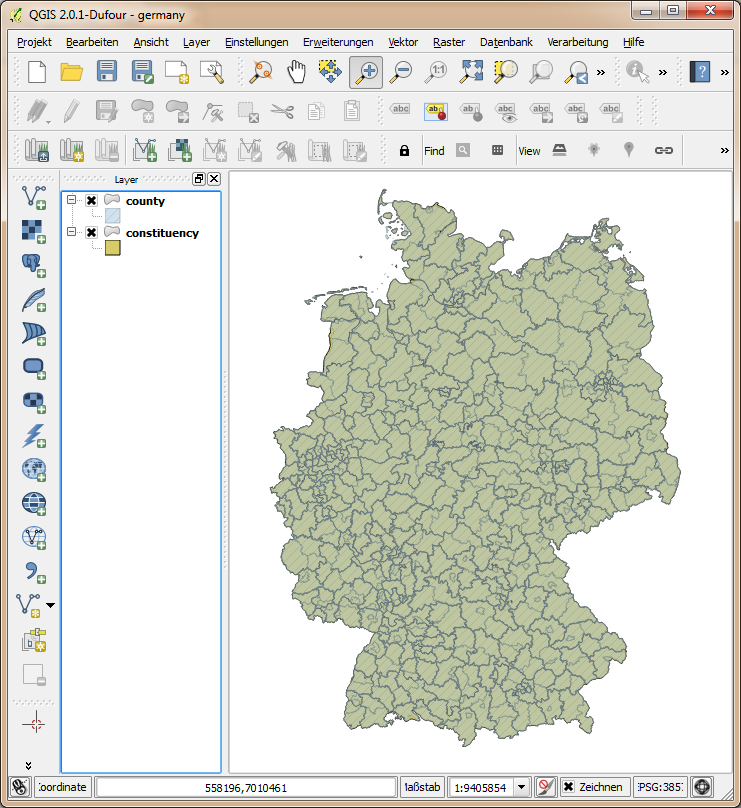
\includegraphics[width=1.1\textwidth]{../img/K4GjcyV.png}
\caption{Wahlkreise and Landkreise merged inside QGIS}
\label{WahlkreiseNLandkreise1}
\end{figure}

\subsubsection{Issues}\label{issues}

A problem occuring with Landkreise (counties) and Wahlkreise (constituencies)
is, as described in the introduction, that both do not have the same borders.
This can be clearly seen in comparision figure \ref{WahlkreisVLandkreis}.

\begin{figure}[htbp]
\centering
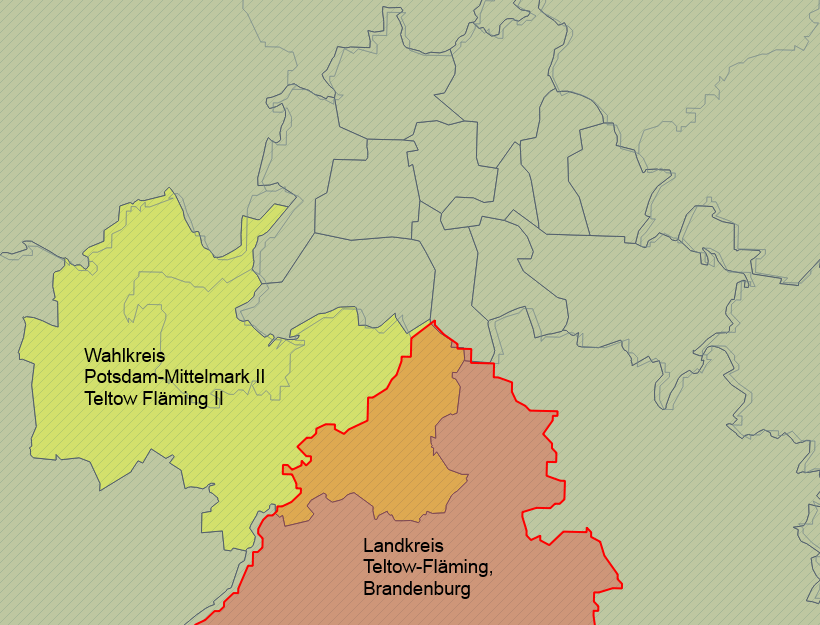
\includegraphics[width=1.1\textwidth]{../img/HdnNLcV.png}
\caption{Wahlkreis (constituency) next to Landkreis (county)}
\label{WahlkreisVLandkreis}
\end{figure}

\begin{enumerate}
\def\labelenumi{\arabic{enumi}.}
\itemsep1pt\parskip0pt\parsep0pt
\item
  \emph{Wahlkreise} and \emph{Landkreise} are not dependent, thus their
  areas are freely intersecting each other.
\item
  \emph{Wahlkreise} and \emph{Landkreise} show a different degree of
  accuracy in position and detail when it comes to border polygons.
\end{enumerate}

\subsection{Setup for Postgres
(+Postgis)}\label{setup-for-postgres-postgis}

\begin{enumerate}
\def\labelenumi{\arabic{enumi}.}
\itemsep1pt\parskip0pt\parsep0pt
\item
  Import shapefiles to the database \emph{public} schema.
\end{enumerate}

\begin{itemize}
\itemsep1pt\parskip0pt\parsep0pt
\item
  \emph{Landkreise} -\textgreater{} ``county''
\item
  \emph{Wahlkreise} -\textgreater{} ``constituency''
\end{itemize}

\begin{enumerate}
\def\labelenumi{\arabic{enumi}.}
\setcounter{enumi}{1}
\itemsep1pt\parskip0pt\parsep0pt
\item
  Add two materialized SQL-Views (virtual tables) for intersections /
  dependencies between ``county'' and ``constituency'':
\end{enumerate}

\begin{lstlisting}[language=SQL]
-- delete old view
DROP MATERIALIZED VIEW IF EXISTS public.county_intersecting_constituency;

-- create area intersection view
CREATE MATERIALIZED VIEW public.county_intersecting_constituency AS 

 WITH intersections AS (
  SELECT lk.id_3 AS county_id,
	wktrns.wkr_nr AS constituency_id,
	CONCAT(lk.name_3, ' (', lk.name_1, ', ', lk.name_2, ')') AS county_label,
	wktrns.wkr_name AS constituency_label,
	ST_AREA(ST_INTERSECTION(ST_SetSRID(lk.geom,4326), wktrns.shape)::geography) AS area_intersection,
	ST_AREA(ST_SetSRID(lk.geom,4326)::geography) AS area_county,
	ST_AREA(wktrns.shape::geography) AS area_constituency
  FROM
	county lk
	JOIN (select wkr_nr, wkr_name, ST_Transform(ST_SetSRID(geom,3044), 4326) AS shape FROM constituency) AS wktrns
	ON ST_INTERSECTS(ST_SetSRID(lk.geom,4326), wktrns.shape))
	
 SELECT
	county_id,
	constituency_id,
	county_label,
	constituency_label,
	area_intersection,
	area_intersection / ((SELECT SUM(i.area_intersection) FROM intersections i WHERE i.county_id = intersections.county_id)) AS area_quota,
	area_county,
	area_constituency
 FROM intersections;

CREATE UNIQUE INDEX county_intersecting_constituency_unique
  ON public.county_intersecting_constituency (county_id, constituency_id);
\end{lstlisting}

\subsection{Derivation of \emph{County} \textless{}-\textgreater{}
\emph{Constituency}}\label{derivation-of-county---constituency}

Take \emph{Berlin} for example:

\begin{lstlisting}[language=SQL]
select * from county_intersecting_constituency where county_label like '%Berlin%' order by area_intersection;
\end{lstlisting}

This request results in a join of intersecting counties and
constituencies, with information about the area of the participate
county, constituency and of course the intersection. A normalized
intersection \textbf{``quota''} index is calculated, which defines the
areal influence of a constituency to a county. The sum of all
constituency ``quota'' of a county is 1.

\begin{table}[h]
\scalebox{0.5}{
\begin{tabular}{|c|c|l|l|r|r|r|r|}
\hline\textbf{county\_id} & \textbf{constituency\_id} & \textbf{county\_label} & \textbf{constituency\_label} & \textbf{area\_intersection} & \textbf{area\_quota} & \textbf{area\_constituency} & \textbf{area\_county} \\ \hline 
141	  &	58    		 &	"Berlin"     &	"Oberhavel Havelland II"	 &	  2803665.490080   &	0.00316685814074   &	2472931758.37186   &	885316816.471166 \\ 
141	  &	63    		 &	"Berlin"     &	"Frankfurt (Oder) Oder-{[}...{]}"   &	  5752379.328977   &	0.00649755449466   &	2405885789.94363   &	885316816.471166 \\ 
141	  &	61    		 &	"Berlin"     &	"Potsdam Potsdam-Mittel{[}...{]}"   &	  6948676.937887   &	0.00784882298049   &	 727030312.23901   &	885316816.471166 \\ 
141	  &	62    		 &	"Berlin"     &	"Dahme-Spreewald Teltow{[}...{]}"   &	  8343997.350849   &	0.00942489609776   &	3973353611.91130   &	885316816.471166 \\ 
141	  &	59    		 &	"Berlin"     &	"M\"arkisch-Oderland Barn{[}...{]}"   &	  8982614.974483   &	0.01014624157473   &	2864879802.60181   &	885316816.471166 \\ 
141	  &	83    		 &	"Berlin"     &	"Berlin-Friedrichshain-K{[}...{]}"   &	 28018823.320075   &	0.03164843988671   &	  28018823.32007   &	885316816.471166 \\ 
141	  &	75    		 &	"Berlin"     &	"Berlin-Mitte"			 &	 45474155.779447   &	0.05136497236676   &	  45474155.77944   &	885316816.471166 \\ 
141	  &	82    		 &	"Berlin"     &	"Berlin-Neuk\"olln"	   	 &	 50038162.639312   &	0.05652021015447   &	  51552590.88985   &	885316816.471166 \\ 
141	  &	81    		 &	"Berlin"     &	"Berlin-Tempelhof-Sch\"one{[}...{]}"   &	 50911846.188703   &	0.05750707248545   &	  52138379.69080   &	885316816.471166 \\ 
141	  &	86    		 &	"Berlin"     &	"Berlin-Lichtenberg"		 &	 54387933.428961   &	0.06143345928648   &	  54578186.82576   &	885316816.471166 \\ 
141	  &	85    		 &	"Berlin"     &	"Berlin-Marzahn-Hellersd{[}...{]}"   &	 55587278.018553   &	0.06278816946519   &	  56213685.87850   &	885316816.471166 \\ 
141	  &	80   		 &	"Berlin"     &	"Berlin-Charlottenburg-W{[}...{]}"   &	 64557831.259508   &	0.07292078680438   &	  64557831.25950   &	885316816.471166 \\ 
141	  &	78   		 &	"Berlin"     &	"Berlin-Spandau Charlot{[}...{]}"   &	 70910610.225396   &	0.08009651795193   &	  83642855.89283   &	885316816.471166 \\ 
141	  &	77    		 &	"Berlin"     &	"Berlin-Reinickendorf"		 &	 77263528.269943   &	0.08727240619467   &	  84103703.05926   &	885316816.471166 \\ 
141	  &	76    		 &	"Berlin"     &	"Berlin-Pankow"			 &	 90999372.170865   &	0.10278761984321   &	  95504666.59105   &	885316816.471166 \\ 
141	  &	79    		 &	"Berlin"     &	"Berlin-Steglitz-Zehlend{[}...{]}"   &	102307387.695839   &	0.11556049918550   &	 106561169.57164   &	885316816.471166 \\ 
141	  &	84    		 &	"Berlin"     &	"Berlin-Treptow-K\"openick"	 &	162026255.436742   &	0.18301547308679   &	 167319473.44736   &	885316816.471166 \\  \hline 
             
\end{tabular}
}
\end{table}


\emph{Notice:} Since the map data of constituencies and counties are
inaccurately overlapping a part of \emph{Brandenburg} constituencies
intersect with the county \emph{Berlin}. The sum of all
\textbf{``quota''} from \emph{Brandenburg} constituencies in
\emph{Berlin} county is 0.03708, which means 3.7\% of \emph{Berlin}s
area will be influenced by voting results descending from constituency
of \emph{Brandenburg}.

